\documentclass[main]{subfiles}

\begin{document}

\begin{frame}
\frametitle{Mathematica Experiments}
Some crazy things I did in Mathematica.
\end{frame}

\begin{comment}
\begin{frame}

  \frametitle{Contents}
  \tableofcontents[currentsection]
\end{frame}


\section{Something}

\frame{

  \frametitle{Evolving Virtual Creatures}
  
  \begin{columns}
   \column{0.3\textwidth}
 \begin{itemize}
	     \item a
    	\item b
    	\item c
     \end{itemize}
     
     \column{0.6\textwidth}
      %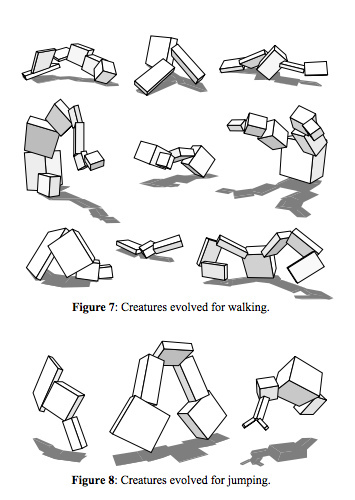
\includegraphics[width=2in, clip] {figs/creatures.jpg} 
  \end{columns}
  }
\note{}

\begin{frame}
\textbf{New colors and their names\\}
Here we show the different colors you can use. From left to right, this are the colors ETH1, ETH2, \ldots , ETH9.

\newcommand{\quadrat}{(0,0mm)--(0mm,5mm)--(5mm,5mm)--(5mm,0mm)--(0mm,0mm);}
\begin{center}
	\hspace{-8mm}
	\begin{tikzpicture}[overlay]
		{\draw[ETHa,fill=ETHa] \quadrat}\label{ETH1}
	\end{tikzpicture}
	\hspace{10mm}
	\begin{tikzpicture}[overlay]
		{\draw[ETHb,fill=ETHb]\quadrat}\label{ETH2}
	\end{tikzpicture}
	\hspace{10mm}
	\begin{tikzpicture}[overlay]
		{\draw[ETHc,fill=ETHc]\quadrat}\label{ETH3}
	\end{tikzpicture}
	\hspace{10mm}
	\begin{tikzpicture}[overlay]
		{\draw[ETHd,fill=ETHd] \quadrat}\label{ETH4}
	\end{tikzpicture}
	\hspace{10mm}
	\begin{tikzpicture}[overlay]
		{\draw[ETHe,fill=ETHe] \quadrat}\label{ETH5}
	\end{tikzpicture}
	\hspace{10mm}
	\begin{tikzpicture}[overlay]
		{\draw[ETHf,fill=ETHf] \quadrat}\label{ETH6}
	\end{tikzpicture}
	\hspace{10mm}
	\begin{tikzpicture}[overlay]
		{\draw[ETHg,fill=ETHg] \quadrat}\label{ETH7}
	\end{tikzpicture}
	\hspace{10mm}
	\begin{tikzpicture}[overlay]
		{\draw[ETHh,fill=ETHh] \quadrat}\label{ETH8}
	\end{tikzpicture}
	\hspace{10mm}
	\begin{tikzpicture}[overlay]
		{\draw[ETHi,fill=ETHi] \quadrat}\label{ETH9}
	\end{tikzpicture}
\end{center}

Please use no more then two of them in your presentation. The first two (counted from the left hand side) are reserved for the administration chapter of the ETHZ (first one for external presentation, second for internal), all others you can freely choose.

\end{frame}

\begin{frame}
\textbf{Some mathematical specialities}

\ETHbox{0.8\textwidth}{% define the ETHbox
  \begin{theorem}[Murphy (1949)]\label{murphy}
    Anything that can go wrong, will go wrong.
  \end{theorem}
}

\begin{proof}
  A special case of Theorem \ref{murphy} is proven in %\citet{matthews1995}.
\end{proof}
\end{frame}

\begin{titlestyleframe}
\frametitle{Title Page}

\color{white} The title page is created using the \texttt{\textbackslash titleframe} command.

The title page background can also be used on other frames (or for a customised title frame) using the \texttt{titlestyleframe} environment.
\end{titlestyleframe}

\begin{frame}
\frametitle{Normal Frame}
The normal frame looks like this. It is created using the \texttt{frame} environment.
\end{frame}

\begin{inverseframe}
  \frametitle{Inverse Slides}
  %\color{white}
The inverted frame looks like this. It is created using the \texttt{inverseframe} environment.
\end{inverseframe}

\begin{minimalframe}
  \frametitle{Minimal Frame}
The minimal frame looks like this. It is created using the \texttt{minimalframe} environment.
  
\end{minimalframe}

\end{comment}

\end{document}